\documentclass[11pt, oneside]{article} 
\usepackage{geometry}
\geometry{letterpaper} 
\usepackage{graphicx}
	
\usepackage{amssymb}
\usepackage{amsmath}
\usepackage{parskip}
\usepackage{color}
\usepackage{hyperref}

\graphicspath{{/Users/telliott_admin/Tex/png/}}
% \begin{center} 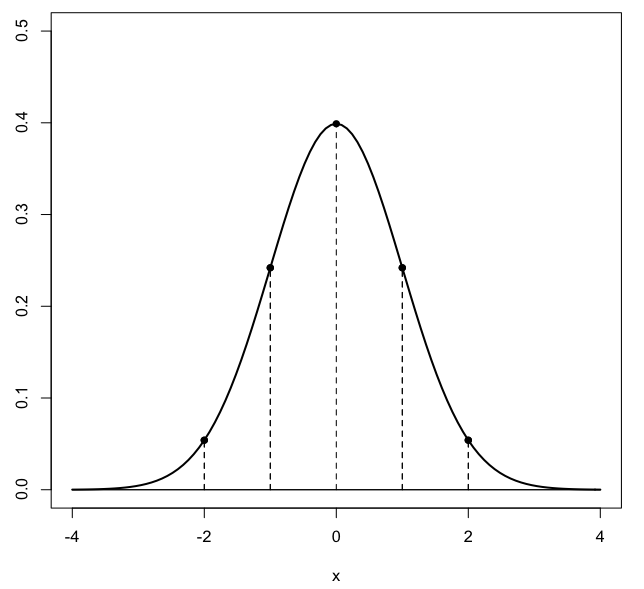
\includegraphics [scale=0.4] {gauss3.png} \end{center}

%break
\title{Euler's equation}
\date{}

\begin{document}
\maketitle
\Large

\label{sec:Euler_quickly}
According to the historians, Newton came up with a series for $e^x$ about 1669 in his book \emph{De analysi per aequationes numero terminorum infinitas}, although he didn't call $e$ by that name or anything.

Recall that one definition of the exponential is
\[ y = e^x = y'  \]
We try to \emph{approximate} this function by a series.  At $x = 0$, $e^x = e^0 = 1$ so
\[ y = 1 \]
So far so good.  However, the derivative $y'$ is then zero.  How do we get a $1$ into the derivative?  By adding a term of $x$
\[ y = 1 + x \]
Now the derivative matches in its first term
\[ y' = 1 \]
But we also need 
\[ y' = y = 1 + x \]
and that $x$ has to come from somewhere in the expression for $y$.  So add $x^2/2$ because its derivative is just $x$ and we obtain
\[ y = 1 + x + \frac{x^2}{2} \]
and again we need 
\[ y' = y = 1 + x + \frac{x^2}{2} \]
so
\[ y = 1 + x + \frac{x^2}{2} + \frac{x^3}{3!} \]
Well, you get the idea.  This continues forever.

There are also infinite series for sine and cosine, of course.  The have traditionally been attributed to Newton, who described them in the work cited earlier.

According to Stewart (\emph{Significant Figures}), they were known much earlier, discovered by the Indian mathematician, Madhava (approximately 1350-1425 C.E.).

\[ \sin x = x - \frac{x^3}{3!} + \frac{x^5}{5!} \dots \]
\[ \cos x = 1 - \frac{x^2}{2!} + \frac{x^4}{4!} \dots \]

Clearly, the derivative of the first series for sine is equal (term by term) to the series for cosine.  And the derivative of the sine is minus the cosine.  It all checks.

Actually, we can use what we know about the derivatives of sine and cosine to follow an approach similar to that for the exponential, to come up with these series ourselves. 

In particular, we know that the second derivative is minus the function, and the fourth derivative is the function itself.
\[ \sin x = \]
The first term can't be $1$ because $\sin 0 = 0$ so write
\[ \sin x = x + \dots \]
Now, we want $\sin'' x = - \sin x$ so
\[ \sin x = x - \frac{x^3}{3!} + \dots \]
does that.  Then $\sin'''' x = \sin x$ so
\[ \sin x = x - \frac{x^3}{3!} + \frac{x^5}{5!} + \dots \]
Then just take the derivative of this to get the series for cosine.

\subsection*{noticing a connection}

Here is a portrait of Euler where he is not wearing that silly hat.

\begin{center} 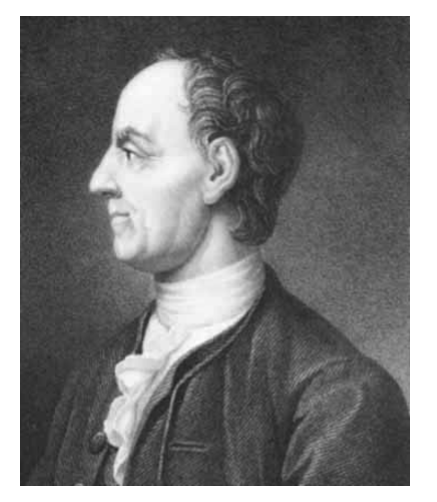
\includegraphics [scale=0.4] {euler.png} \end{center}

Euler said, let us consider the complex number
\[ z = \cos \theta + i \sin \theta \]

How in the world did he come up with this?  Perhaps because he already knew the answer.  

My guess is that he looked at the formula
\[ e^x = \sum_{n=0}^{\infty} \frac{x^n}{n!}  =  1 + x + \frac{x^2}{2!} + \frac{x^3}{3!} + \frac{x^4}{4!} \dots \]
and said:  it cannot be an accident that the sine and cosine series look so similar, in fact when added together they have exactly the same terms, just with some periodically occuring minus signs.

\[ \sin x + \cos x = 1 + x - \frac{x^2}{2!} - \frac{x^3}{3!} + \frac{x^4}{4!} + \frac{x^5}{5!} \dots \]

Where would I get alternating plus and minus signs from?  Maybe if I substitute $ix$ for $x$?
\[ e^{ix} = \sum_{n=0}^{\infty} \frac{{ix}^n}{n!}  =  1 + ix - \frac{x^2}{2!} -  i\frac{x^3}{3!} + \frac{x^4}{4!} \dots \]

Clearly, part of this is
\[ \cos x = 1 - \frac{x^2}{2!} + \frac{x^4}{4!} - \frac{x^6}{6!} \dots \]
while the rest is
\[ ix -  i\frac{x^3}{3!} + i\frac{x^5}{5!}\dots = i \sin x \]

\subsection*{quick and dirty derivation}

Let's just see what we can do. 

 If we assume that calculus is legal with complex numbers (assuming that $i$ is just a number), we can do the following
\[ z = \cos \theta + i \sin \theta \]
\[ \frac{dz}{d \theta} = - \sin \theta + i \cos \theta \]
(It turns out that it is legal, but the argument requires the fact these functions are all \emph{analytical}, which is beyond our scope here).

And since $i^2 = -1$
\[ \frac{dz}{d \theta} = i^2 \sin \theta + i \cos \theta \]
\[ \frac{dz}{d \theta} = i(i \sin \theta + \cos \theta) = iz \]

Rearrange
\[ \frac{1}{z} \ dz = i \ d \theta \]
\[ \int \frac{1}{z} \ dz = \int i  \ d \theta \]
\[ \ln z = i \theta \]
Exponentiate:
\[ z = e^{i \theta} \]
\[ e^{i \theta} = \cos \theta + i \sin \theta \]

Euler's famous result in a few lines, which he proved more rigorously (but not completely so) by other approaches explored \hyperref[sec:Euler's_equation]{\textbf{here}}.

\subsection*{addendum}
We've really gone fast and loose in this section.  One thing that makes series hard is that a series is sometimes valid only for a certain range of $x$.  Consider
\[ \frac{1}{1 - x} = 1 + x + x^2 + x^3 + x^4 \dots \]
The equality is easily verified if you multiply both sides by $1 - x$.  You get the right-hand side, plus a version of the right hand side containing every term except the first, all with minus signs.  It all adds up to $1$.
 
The problem is, the series is obviously not valid for $x = 1$, nor for $x > 1$.  Consider $x = 2$.  (It gets worse.  Consider $x = -1$).  In fact, it turns out to be valid only for $|x| < 1$, which is called the radius of convergence.

Luckily, the exponential series and those for sine and cosine \emph{are} valid for all $x$.

According to Nahin (\emph{An Imaginary Tale}), both Abraham de Moivre and Roger Cotes knew Euler's identity decades before he published it.  Which may be a good example of

\url{https://en.wikipedia.org/wiki/Stigler%27s_law_of_eponymy}

\end{document}